\documentclass[11pt,a4paper]{article}

\usepackage[utf8]{inputenc}
\usepackage[T1]{fontenc}
\usepackage[french]{babel}
\usepackage[a4paper,margin=2.2cm]{geometry}
\usepackage{graphicx}
\usepackage{amsmath}
\usepackage{amssymb}
\usepackage{booktabs}
\usepackage{hyperref}
\usepackage{listings}
\usepackage{xcolor}
\usepackage{caption}

\hypersetup{
  colorlinks=true,
  linkcolor=black,
  urlcolor=blue!60!black,
  citecolor=black,
}

\lstdefinestyle{python}{
  basicstyle=\ttfamily\scriptsize,
  keywordstyle=\color{blue!70!black}\bfseries,
  stringstyle=\color{green!50!black},
  commentstyle=\color{gray}\itshape,
  numbers=left,
  numberstyle=\tiny\color{gray},
  frame=single,
  breaklines=true,
  language=Python,
  showstringspaces=false,
}

\title{\textbf{Rapport individuel} \\
       \large Mini-Projet GANs et Diffusion \\
       Contribution : Dataset Fashion-MNIST et generation avec un GAN}
\author{Dylan Peltier \\ M2 IA \& Big Data --- ESIEE-IT Pontoise}
\date{2025--2026}

\begin{document}

\maketitle

\section{Perimetre de la contribution}

Le mini-projet est decoupe en quatre parties techniques (dataset, GAN, diffusion, comparaison/erreurs) et une partie d'analyse critique. Ma contribution couvre les deux premieres parties : la mise en place du \textbf{dataset Fashion-MNIST} et l'implementation complete d'un \textbf{GAN} pour la generation d'images de cette base. Les artefacts que je transmets aux autres membres du groupe sont :

\begin{itemize}
    \item un pipeline de chargement et de pretraitement reproductible (\texttt{seed=42}, normalisation $[-1, 1]$);
    \item les poids du generateur et du discriminateur (\texttt{gan\_generator.pth}, \texttt{gan\_discriminator.pth});
    \item un lot de 100 images generees (\texttt{gan\_images\_for\_analysis.pth}) qui sert d'entree a la partie comparaison et a l'etude des erreurs.
\end{itemize}

\section{Section Dataset --- Fashion-MNIST}

\subsection{Choix et caracteristiques}

Fashion-MNIST est un dataset de 70~000 images en niveaux de gris, de taille $28 \times 28$ pixels, reparties en 10 classes vestimentaires : T-shirt, Pantalon, Pull, Robe, Manteau, Sandale, Chemise, Sneaker, Sac et Bottine. Le split standard fournit 60~000 images d'entrainement et 10~000 images de test. C'est le dataset preconise par la fiche de projet : il est leger (entrainement realiste sur GPU grand public), accessible directement via \texttt{torchvision.datasets.FashionMNIST}, et structurellement plus riche que MNIST chiffres, ce qui permet d'observer de vraies pathologies generatives (mode collapse, hybridation de classes).

\subsection{Pipeline implemente}

J'ai concu un pipeline minimal et reproductible :

\begin{lstlisting}[style=python,caption={Pretraitement Fashion-MNIST}]
transform = transforms.Compose([
    transforms.ToTensor(),
    transforms.Normalize((0.5,), (0.5,)),  # [-1, 1] pour matcher Tanh
])
\end{lstlisting}

\noindent Le choix d'une normalisation $[-1, 1]$ n'est pas neutre : il est dicte par la sortie \texttt{Tanh} du generateur (section suivante). Une normalisation $[0, 1]$ aurait force a utiliser une \texttt{Sigmoid} en sortie du generateur, qui est notoirement moins stable a l'entrainement d'un GAN. Cette coherence entre la normalisation du dataset et l'activation de sortie du generateur est une condition tacite mais essentielle.

\subsection{Verification quantitative}

Le batch echantillonne respecte la specification : valeurs dans $[-1.0, 1.0]$ exactement, moyenne $\approx -0.43$ (logique : la majorite des pixels sont en noir, valeur $-1$), ecart-type $\approx 0.70$. La figure~\ref{fig:dataset} montre la distribution des classes et un echantillon. Le dataset est \emph{parfaitement equilibre} (6~000 images de train et 1~000 de test par classe), donc aucun reweighting n'est necessaire.

\begin{figure}[h]
    \centering
    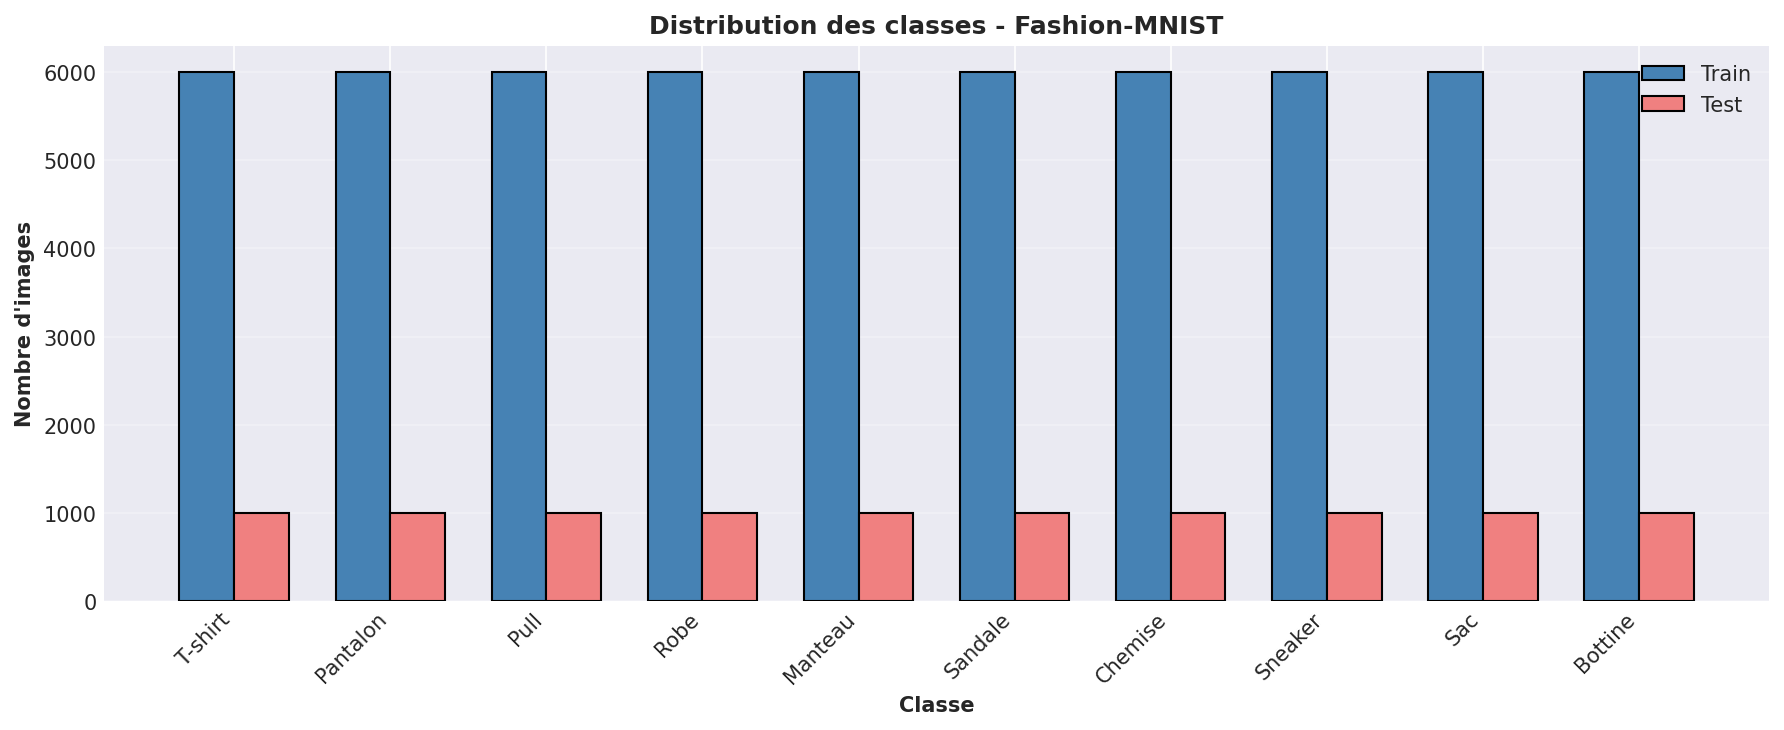
\includegraphics[width=\linewidth]{02_distribution_classes.png}
    \caption{Distribution des classes Fashion-MNIST : 6~000 (train) et 1~000 (test) par classe.}
    \label{fig:dataset}
\end{figure}

\subsection{Analyse des difficultes anticipees}

\paragraph{Classes difficiles a generer.} La similarite inter-classes est le principal danger : T-shirt, Pull, Chemise et Manteau partagent la meme silhouette de base (corps + manches), ce qui pousse un modele non conditionne a produire des images intermediaires non identifiables. A l'inverse, les classes structurellement separees dans l'espace des images (Pantalon, Sandale, Sac) sont plus simples a generer.

\paragraph{Details visuels delicats.} A $28 \times 28$ en niveaux de gris, les details suivants sont sous-representes en signal et faciles a degrader : lacets de chaussures, sangles de sacs, boutons, cols, mailles tricotees, motifs imprimes. Le modele tend a les remplacer par des zones uniformes.

\paragraph{Difficultes intrinseques pour un modele generatif.} La faible resolution ecrase l'information fine sur tres peu de pixels, ce qui rend la reconstruction de details ambigue. L'absence de couleur supprime un signal discriminant entre classes, et la multi-modalite intra-classe (chaussure de cote, de face, avec talon ou plate) favorise le mode collapse.

\section{Section Partie 1 --- Generation avec un GAN}

\subsection{Choix d'architecture : DCGAN}

J'ai retenu une architecture \textbf{DCGAN} (Radford et al., 2015) adaptee au format $28 \times 28$ plutot qu'un GAN purement dense. Le DCGAN est devenu la baseline canonique pour les images naturelles parce qu'il combine plusieurs choix qui font converger l'entrainement de maniere fiable : convolutions transposees avec strides au lieu d'upsampling explicite, \texttt{BatchNorm} entre couches, \texttt{ReLU} (generateur) / \texttt{LeakyReLU} (discriminateur), pas de couche \emph{fully-connected} a part la projection initiale, et \texttt{Tanh} en sortie.

\paragraph{Generateur.} Projection dense $z \in \mathbb{R}^{100}$ vers un tenseur $7 \times 7 \times 256$, puis deux \texttt{ConvTranspose2d} (stride 2) qui doublent la resolution a chaque etape, $7 \to 14 \to 28$. Chaque couche intermediaire est suivie de \texttt{BatchNorm2d} + \texttt{ReLU}. La sortie est lissee par une \texttt{Conv2d} $3 \times 3$ suivie d'une \texttt{Tanh}. Total : 4{,}88 M parametres.

\paragraph{Discriminateur.} Trois \texttt{Conv2d} avec strides ($28 \to 14 \to 7 \to 4$), \texttt{LeakyReLU(0.2)} et \texttt{BatchNorm2d} entre couches, suivies d'une projection dense vers un logit scalaire. J'utilise \texttt{BCEWithLogitsLoss} plutot que \texttt{Sigmoid + BCELoss} pour la stabilite numerique (la version \texttt{Logits} est numeriquement plus saine quand les logits sont extremes). Total : 1{,}07 M parametres.

\paragraph{Vecteur latent.} J'ai fixe \texttt{latent\_dim = 100}, valeur standard du papier DCGAN. Une dimension inferieure (16--32) tend a limiter la diversite generee ; une dimension superieure (256+) augmente la difficulte d'optimisation sans gain mesurable sur un dataset aussi simple.

\subsection{Hyperparametres et boucle d'entrainement}

\begin{table}[h]
    \centering
    \small
    \begin{tabular}{ll}
        \toprule
        \textbf{Parametre} & \textbf{Valeur} \\
        \midrule
        Dimension latente & 100 \\
        Batch size & 128 \\
        Nombre d'epochs & 50 \\
        Optimiseur & Adam ($\beta_1 = 0{,}5$, $\beta_2 = 0{,}999$) \\
        Learning rate G et D & $2 \times 10^{-4}$ \\
        Loss & \texttt{BCEWithLogitsLoss} (objectif non saturant) \\
        Initialisation & $\mathcal{N}(0, 0{,}02)$ pour Conv et Linear \\
        Seed & 42 (Python, NumPy, PyTorch, CUDA) \\
        \bottomrule
    \end{tabular}
    \caption{Hyperparametres retenus pour l'entrainement du DCGAN.}
\end{table}

A chaque iteration je realise (i) une mise a jour du discriminateur sur \texttt{BCE($D$(reel), 1) + BCE($D$(faux), 0)}, puis (ii) une mise a jour du generateur sur \texttt{BCE($D$(faux), 1)} (objectif non saturant de Goodfellow). Pour suivre l'evolution du generateur de maniere comparable d'une epoch a l'autre, je stocke un snapshot a partir d'un \textbf{bruit fixe} \texttt{fixed\_noise} en fin de chaque epoch ; cela isole l'effet de l'apprentissage de l'effet de l'aleatoire du sampling.

\subsection{Resultats et lecture des courbes}

\begin{figure}[h]
    \centering
    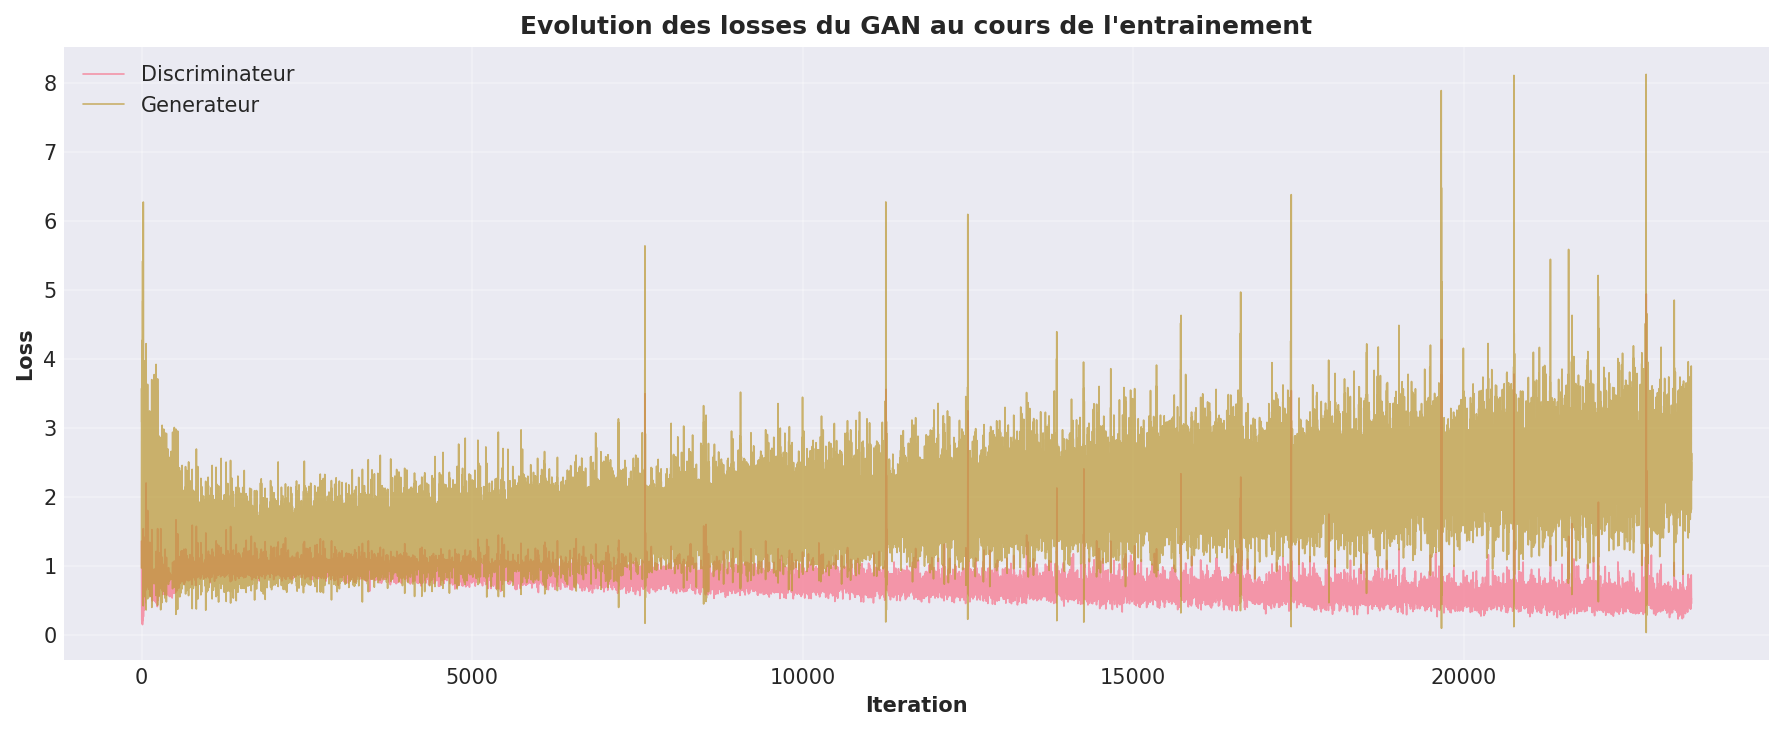
\includegraphics[width=\linewidth]{03_gan_losses.png}
    \caption{Evolution des losses $D$ et $G$ sur l'ensemble de l'entrainement. La D\_loss reste stable autour de 0{,}5--1{,}0, la G\_loss derive de 2 vers 3--4 avec des pics ponctuels au-dela de 6.}
    \label{fig:losses}
\end{figure}

La figure~\ref{fig:losses} montre un patron classique : le discriminateur \emph{prend l'avantage} progressivement. La \texttt{D\_loss} converge vers une zone stable autour de 0{,}5--1{,}0 (rappel : l'equilibre theorique ideal est $2\ln 2 \approx 1{,}39$), tandis que la \texttt{G\_loss} derive a la hausse, de $\approx 2$ en debut a $\approx 3$--$4$ a la fin, avec des pics ponctuels jusqu'a 8. Ces pics ne sont pas des divergences durables : la boucle se restabilise immediatement apres, ce qui indique que le generateur reste capable de tromper le discriminateur la majorite du temps, malgre des episodes courts ou il echoue.

\textbf{Lecon pratique sur les losses GAN.} Contrairement a un classifieur, les losses GAN ne sont pas un proxy de la qualite. Une \texttt{D\_loss} qui chuterait vers 0 serait une mauvaise nouvelle (le discriminateur ecrase le generateur, le gradient du generateur s'eteint) ; une \texttt{G\_loss} qui chuterait brutalement traduirait souvent un mode collapse. Ici, le scenario observe (\texttt{D\_loss} stable, \texttt{G\_loss} en derive douce) est interpretable comme un equilibre encore exploitable mais qui se degrade en faveur du discriminateur --- un entrainement plus long demanderait soit un ratio $D{:}G$ inferieur (mise a jour de $G$ deux fois par iteration), soit du label smoothing pour ralentir $D$.

\begin{figure}[h]
    \centering
    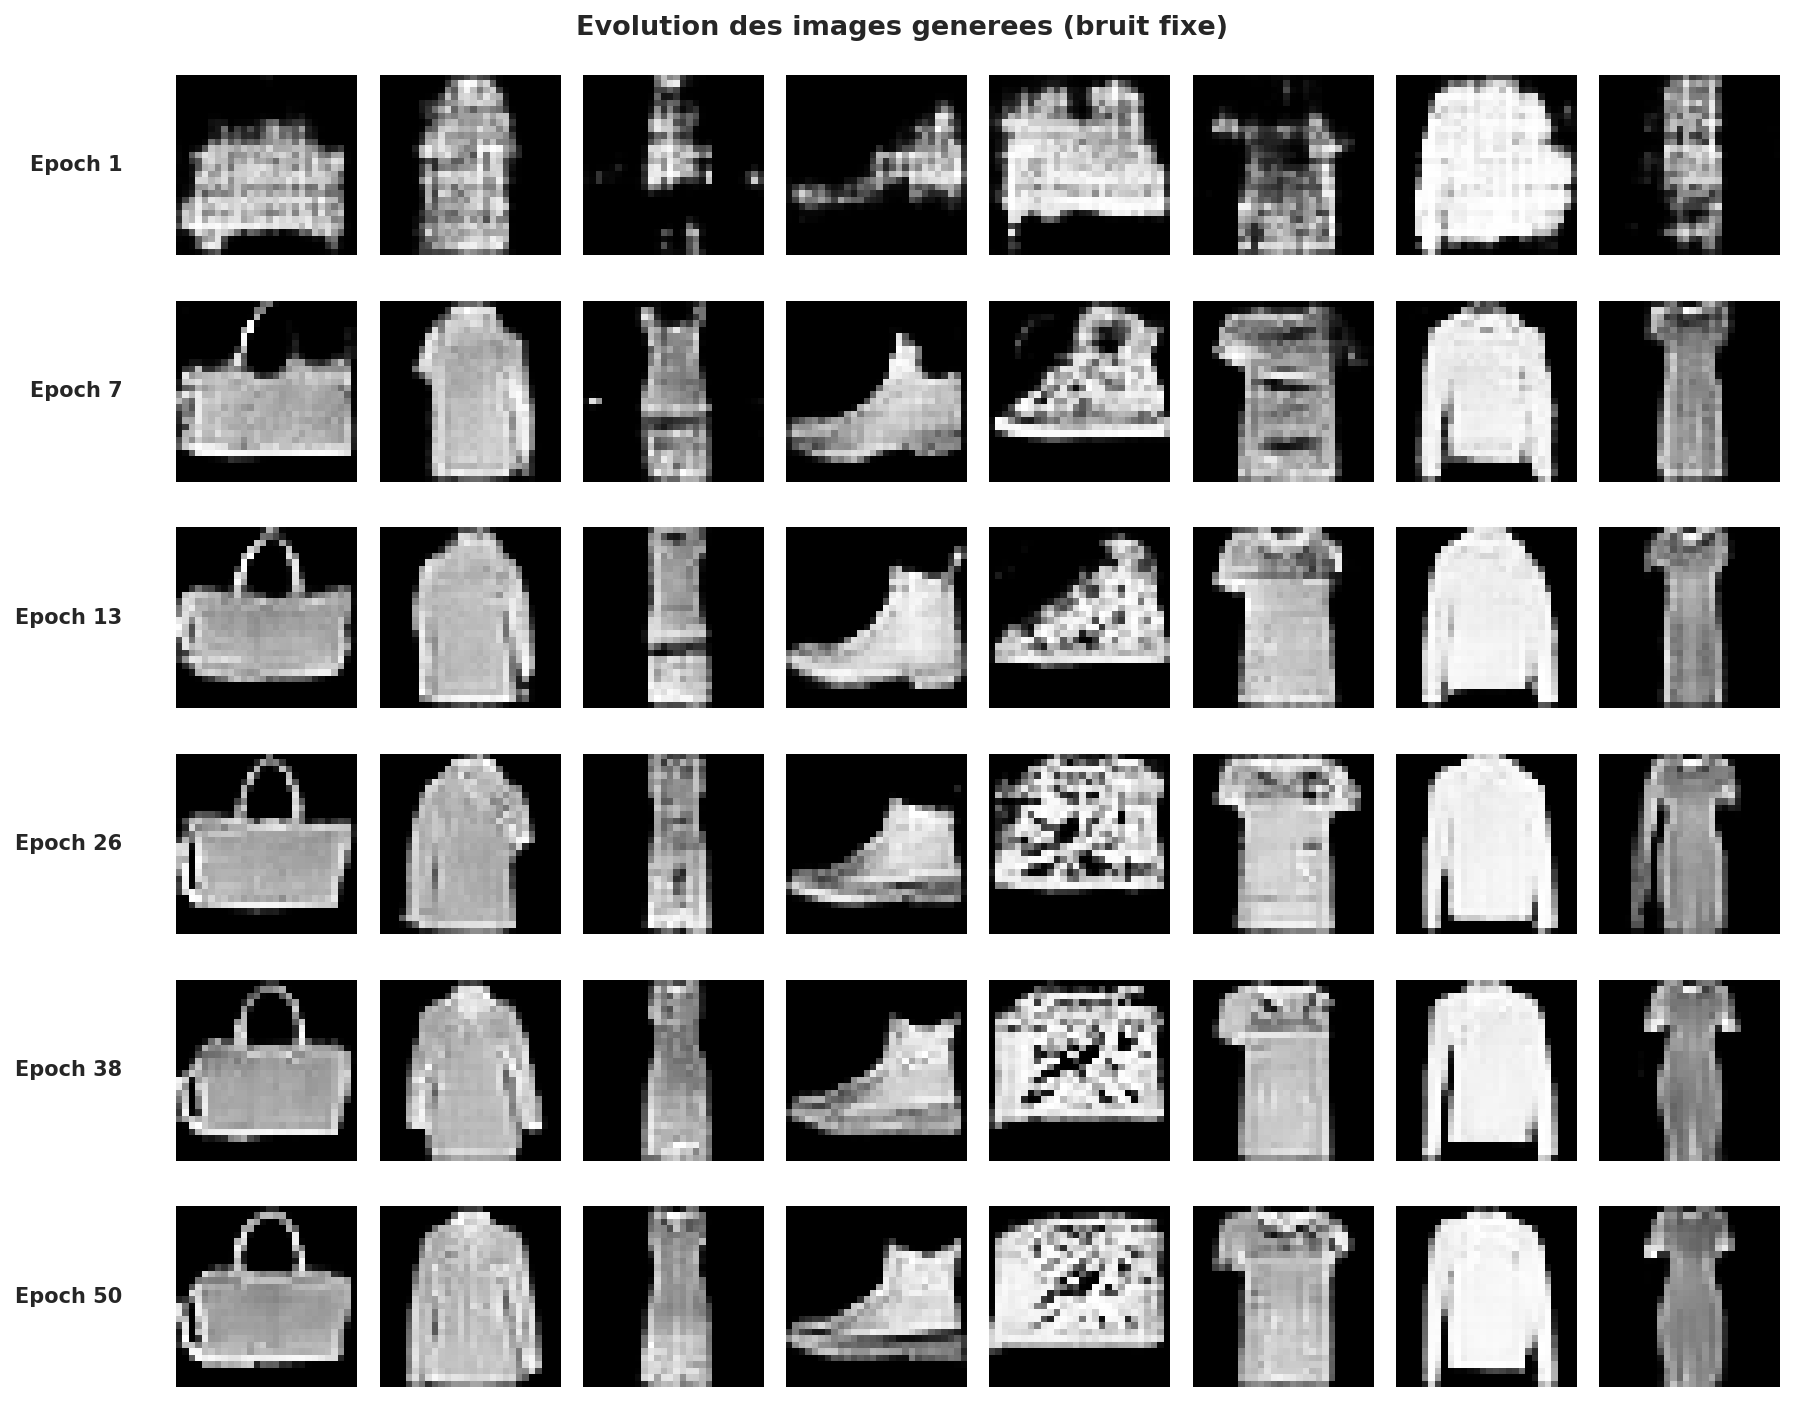
\includegraphics[width=\linewidth]{04_gan_evolution.png}
    \caption{Evolution des images generees a partir du \emph{meme} bruit fixe sur 6 epochs reparties. Seul le generateur change d'une ligne a l'autre.}
    \label{fig:evolution}
\end{figure}

La figure~\ref{fig:evolution} confirme la convergence visuelle : a l'epoch 1, les sorties sont des blobs flous mais possedent deja les axes spatiaux corrects (silhouettes globales esquissees). Des l'epoch 7, sept des huit colonnes affichent des objets identifiables (sac, pull/manteau, robe, bottine, t-shirt, robe). Entre les epochs 13 et 50, le raffinement se concentre sur les bords (silhouette plus nette du sac, contraste accru, structure du col du pull mieux dessinee). Le plafond qualitatif est atteint relativement tot, conforme a ce qu'on attend d'un DCGAN sur ce dataset.

\paragraph{Cas pathologique notable.} La cinquieme colonne de la figure~\ref{fig:evolution} montre un cas typique d'\emph{echec local du generateur}. Le point latent en question donne lieu, au fil des epochs, a une image de plus en plus structuree par un motif damier de haute frequence sans semantique reconnaissable. Le generateur a appris a placer cette texture pour ce vecteur latent precis, mais elle ne correspond a aucune classe de Fashion-MNIST. C'est un sous-cas typique de \emph{mode failure} ponctuel.

\begin{figure}[h]
    \centering
    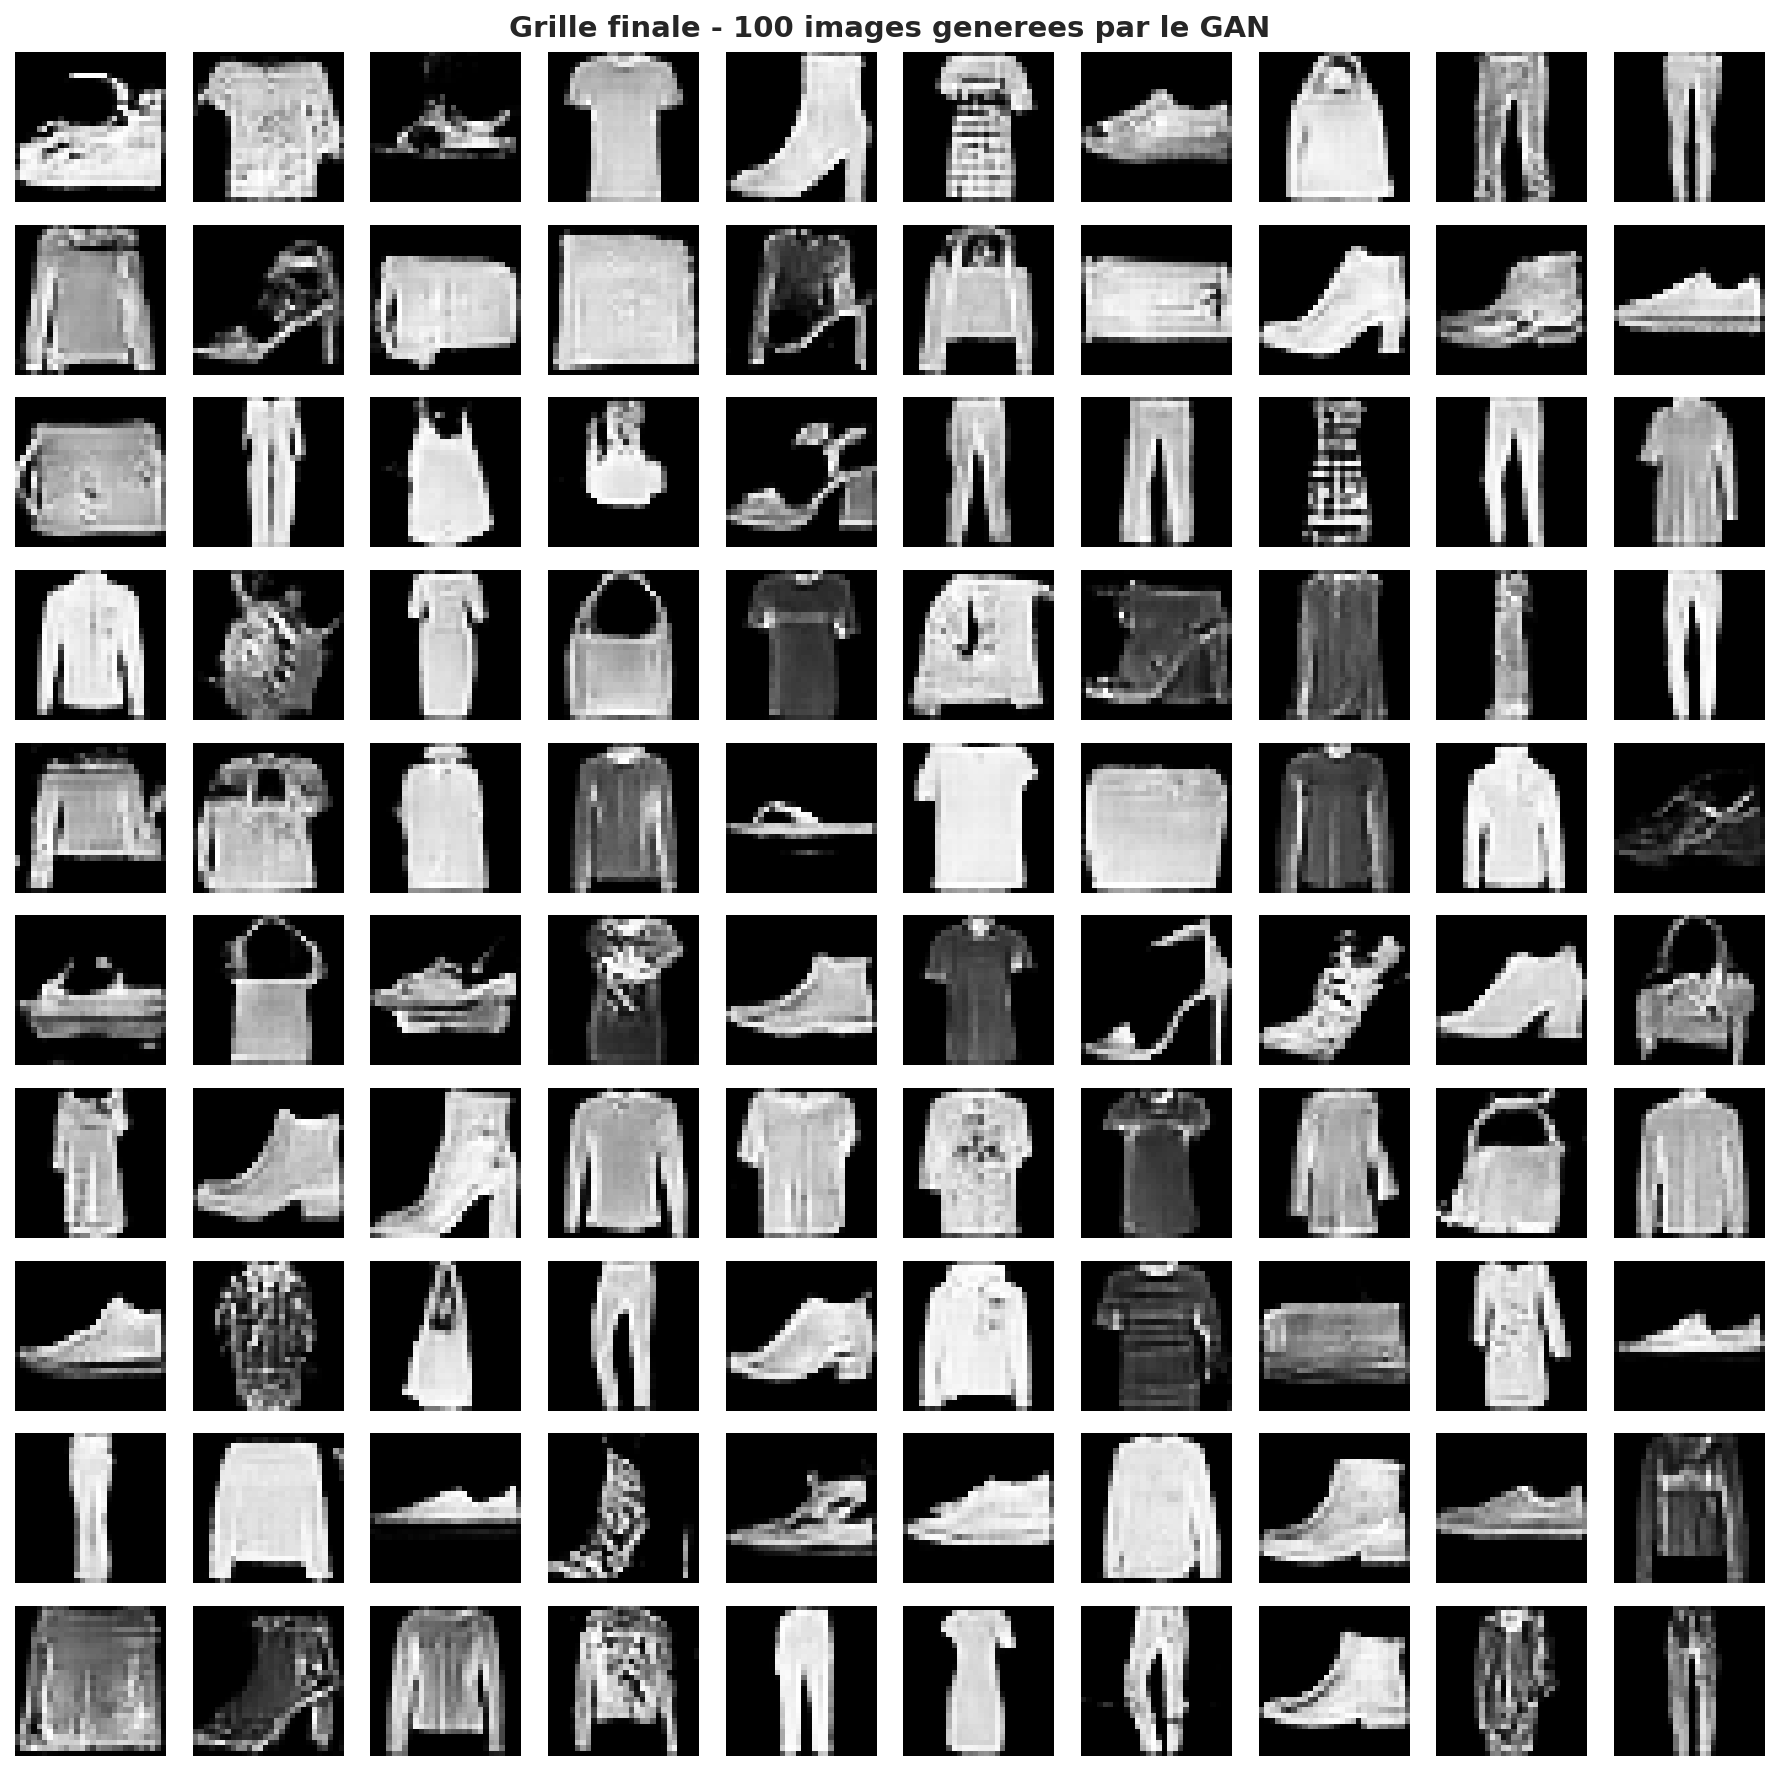
\includegraphics[width=0.85\linewidth]{05_gan_final_grid_100.png}
    \caption{Grille finale : 100 images independantes generees apres entrainement.}
    \label{fig:grid}
\end{figure}

La grille de 100 images (figure~\ref{fig:grid}) montre une diversite reelle : on identifie des sacs, des pantalons, des bottines (de hauteur variable), des sneakers, des chaussures a talon, des hauts et des robes. \textbf{Pas de mode collapse global}, mais des signaux locaux : (i) sur-representation visuelle des classes structurellement simples (silhouette de pantalon, sac), (ii) plusieurs cases qui contiennent des silhouettes hybrides T-shirt/Chemise/Pull non identifiables, (iii) des chaussures avec des bouts mal definis, et (iv) quelques cases tres claires ressemblant a des halos sans structure precise.

\subsection{Reponses aux questions d'analyse}

\paragraph{Realisme au cours de l'entrainement.} Oui, et la transition est tres rapide : entre les epochs 1 et 7, on passe de blobs a des objets identifiables. Les 40 epochs suivantes apportent un raffinement marginal des bords et du contraste.

\paragraph{Diversite.} Correcte mais inferieure a celle du dataset reel. Sur 100 images, je compte plusieurs sacs (au moins 8), des pantalons (au moins 10), des chaussures variees (sneakers, bottines, talons), des hauts varies. Certaines classes (Sandale notamment) sont sous-representees dans les sorties.

\paragraph{Mode collapse.} Pas de collapse total. En revanche des signes locaux : repetitions de silhouettes voisines, et le cas pathologique de la colonne 5 de la figure~\ref{fig:evolution} qui se ``fige'' sur un motif sans contenu semantique.

\paragraph{Defauts les plus frequents.} Flou sur les bords (artefacts caracteristiques des \texttt{ConvTranspose2d} a stride 2), manches et chaussures asymetriques, semelles mal definies, hybridations entre classes proches (T-shirt/Chemise/Pull), et quelques images quasi-uniformes.

\paragraph{Interpretabilite des losses.} Faible. Les losses servent surtout a detecter les pathologies (divergence, ecrasement de $G$, mode collapse). L'evaluation reelle de la qualite passe par l'inspection visuelle ou des metriques specifiques (FID, IS) non implementees dans ce mini-projet.

\section{Bilan et choix techniques}

Trois choix sont a souligner. (1) Avoir adopte la baseline DCGAN plutot qu'une architecture personnalisee m'a permis d'obtenir un entrainement stable des le premier essai, et de me concentrer sur l'analyse plutot que sur le debogage. (2) L'utilisation du \emph{bruit fixe} pour les snapshots est ce qui donne sa valeur diagnostique a la figure~\ref{fig:evolution} : sans cela, on melange l'effet de l'apprentissage et l'effet du sampling, et on ne peut pas distinguer la convergence d'un cas d'echec local. (3) \texttt{BCEWithLogitsLoss} plutot que \texttt{Sigmoid + BCELoss} : c'est un detail d'implementation mais il evite des explosions numeriques quand le discriminateur produit des logits extremes, ce qui arrive frequemment a la fin de l'entrainement (voir les pics de la figure~\ref{fig:losses}).

Le rapport general developpe plus en detail le positionnement de cette partie GAN dans le cadre comparatif global du projet (vs. diffusion).

\end{document}
